%{{{ prelude latex
\tracingmacros=0
\documentclass{llncs}
%{{{ packages
\usepackage[english]{babel}
\usepackage{amsmath}
\usepackage{amssymb}
\usepackage{booktabs}
\usepackage{graphicx}  % TODO: paint everything in tikz and remove this
\usepackage{listings}
\usepackage{mathrsfs}
\usepackage{microtype} % keep even if it seems not to do anything!
\usepackage{tikz}
\usepackage{xcolor}
\usepackage{xspace}
\usepackage[colorlinks]{hyperref}  % solves pdfTeX warning (ext4)?
\usepgflibrary{arrows}
%}}}
%{{{ meta
\def\fbtitle{FreeBoogie}
\def\fbauthors{Radu Grigore and Joseph Kiniry}
\title{\fbtitle}
\author{\fbauthors}
%}}} meta
%{{{ PDF settings
\definecolor{darkblue}{rgb}{0,0,0.4}
\definecolor{verylightgray}{rgb}{0.9,0.9,0.9}
% comment the next line for printing
\hypersetup{colorlinks,linkcolor=darkblue,citecolor=darkblue,urlcolor=darkblue}
\hypersetup{
  pdfauthor={\fbauthors},
  pdftitle={\fbtitle}}
%}}}
%{{{ tikz helpers

% global styles
\tikzstyle{arr}=[->,>=stealth']
\tikzstyle{predcirc}=[
  circle,
  very thick,
  fill=green!10,
  draw=green,
  minimum size=14pt,
  inner sep=0pt]
\tikzstyle{predrect}=[predcirc,rectangle,inner sep=2pt]

% These macros and styles are used for drawing flowgraphs
\newcommand\fgnodeR{2pt}  % the default radius of a flowgraph node
\tikzstyle{fgdraw}=[
  minimum size=2*\fgnodeR,inner sep=0pt,outer sep=1pt,
  draw,thick]
\tikzstyle{fgfill}=[fill=black]
\ifx\fgnode\undefined\else\errmessage{\string\fgnode already defined!}\fi
\def\fgnode#1#2(#3) at (#4){% uses \def because of the special syntax
    \begin{scope}[shift={(#4)},shift only]
      \clip (-\fgnodeR,-#1*\fgnodeR) rectangle (\fgnodeR,#2*\fgnodeR);
      \node[fgdraw,circle,fgfill] {};
    \end{scope}
    \node[fgdraw,circle] (#3) at (#4)}
\newcommand{\oonode}{\fgnode00} % the normal non-reading non-writing node
\newcommand{\ronode}{\fgnode01} % for read-only nodes
\newcommand{\wonode}{\fgnode10} % for write-only nodes
\newcommand{\rwnode}{\fgnode11} % for read-write nodes
\newcommand{\gnode}{\node[fgdraw,circle,fill=gray]}  % gray nodes (ra)
\newcommand{\cnode}{\node[fgdraw,fgfill,rectangle]} % copy nodes
\newcommand{\enode}{\oonode} % empty node
\newcommand{\fnode}{\rwnode} % filled node
%}}}
%{{{ package customization
\lstset{
  basicstyle=\scriptsize,
  identifierstyle=\itshape,
  stringstyle=\footnotesize\ttfamily,
  commentstyle=\textup,
  columns=fullflexible,
  numbers=left,
  numberstyle=\tiny,
  mathescape=true,
  boxpos=t,
}
\lstdefinestyle{boogie}{
  morekeywords={procedure,returns,assume,assert,havoc,goto,return,
    int,bool,type,while,if,true,false,function,bool,returns,axiom,
    forall,var}
}
\lstdefinestyle{jml}{
  language=java,
  morekeywords={requires,ensures,old,invariant,forall,exists,axiom,also,
    result,pure,assert,modifies},
  deletekeywords={label}
}
\lstdefinestyle{smt}{
  morekeywords={ite,true,false,BG_PUSH,IFF,FORALL,EQ,NEQ,NOT,TRUE,FALSE,
    IMPLIES}
}
\newcommand{\lstinlinen}{\lstinline[basicstyle=\normalsize]}
\newcommand{\boogieCode}{\lstinline[style=boogie,basicstyle=\normalsize]}
\newcommand{\jmlCode}{\lstinline[style=jml,basicstyle=\normalsize]}
\newcommand{\smtCode}{\lstinline[style=smt,basicstyle=\normalsize]}
\newcommand{\deflang}[1]{\lstnewenvironment{#1}[1][]{\lstset{style=#1,##1}}{}}
\deflang{jml}
\deflang{boogie}
\deflang{smt}
\abovetopsep=1ex % because tabular appears below captions
%}}}
%{{{ new commands 
\def\fb#1{{\bf #1}} % for introducing acronyms
\newcommand{\csharp}{C$^\sharp$\xspace}
\newcommand{\escjava}{ESC\slash Java\xspace}
\newcommand{\framac}{\hbox{Frama-C}}
\newcommand{\fx}{F\kern-0.1667em\lower.5ex\hbox{X}\kern-.125em 7\xspace}
\newcommand{\indentline}[1]{\\\leftline{\indent#1}}
\newcommand{\macro}[1]{\texttt{\char`\\#1}}
\newcommand{\jk}[1]{{\small [\textcolor{red}{jk}: #1]}}
\newcommand{\rg}[1]{{\small [\textcolor{red}{rg}: #1]}}
\newcommand{\shell}[1]{\indentline{\texttt{#1}} }
\newcommand{\specsharp}{Spec$^\sharp$\xspace}

%pairs
\newcommand{\startgrammar}{
  \begingroup
  \def\is{&$\to$&}
  \def\|{$\mid$}
  \def\b##1{\textbf{##1}}
  \def\i##1{\textsl{##1}}
  \def\?{$^?$}
  \def\*{$^\ast$}
  \begin{figure}
  \centering
  \scriptsize
  \begin{tabular}{r@{\;}c@{\;}l}
}
\newcommand{\stopgrammar}[2]{
  \end{tabular}
  \caption{#1}\label{#2}
  \end{figure}
  \endgroup
}

\newcommand{\bc}{\begin{figure}\centering\begin{tabular}{c}} % begin codebox
\newcommand{\ec}[2]{\end{tabular}\caption{#1}\label{#2}\end{figure}} % end codebox

%}}}
%{{{ new environments (and theorems)
% TODO: Get rid of these. This should be a non-mathy `tool paper'.
%\newtheoremstyle{slanted}{}{}{\slshape}{}{\bf}{.}{.5em}{}
%\theoremstyle{slanted}
%\newtheorem{problem}{Problem}
%\newtheorem{conjecture}{Conjecture}
%\newtheorem{lemma}{Lemma}
%\newtheorem{proposition}{Proposition}
%\newtheorem{theorem}{Theorem}
%\newtheorem{corollary}{Corollary}
%\theoremstyle{definition}
%\newtheorem{definition}{Definition}
%\newtheorem{example}{Example}
%\theoremstyle{remark}
%\newtheorem{remark}{Remark}
%}}}
%{{{ TeX settings
\overfullrule=5pt
\showboxdepth=10
\showboxbreadth=100
%}}}
%}}}

\begin{document}
\maketitle
% {{{ abstract
\begin{abstract}

There are many verification condition generators, each with its own design.
This article documents the main design decisions of FreeBoogie.
It is 

Researchers often implement VCGENs (\fb verification \fb condition
\textbf{gen}erators) as part of their experiments. Certain design
principles keep being rediscovered. This article summarizes a few lessons
that the authors learned by developing one VCGEN and by studying many
others.

\end{abstract}
% }}} abstract
%{{{ run
\section{An Example Run}

\bc
\begin{boogie}
type T;
procedure indexOf(x : T, a : [int] T, al : int) returns (i : int) {
  i := 0;
  while (i < al && a[i] != x) { i := i + 1; }
}
\end{boogie}
\ec{A high-level Boogie version of Figure~\ref{lst:first-boogie}}
{lst:boogie-indexof}

The best way to understand how FreeBoogie works is to run
it on a few examples and ask it to dump its data structures
at intermediate stages. Figure~\ref{lst:boogie-indexof}
shows a Boogie program suitable for a first run. Notice
that the language is not restricted to the core defined in
Chapter~\ref{ch:boogie}. To peek at FreeBoogie's internals
use the command \shell{fb --dump-intermediate-stages=log
example.bpl} assuming that you wrote the content of
Figure~\ref{lst:first-boogie} in the file \texttt{example.bpl}
and that FreeBoogie is correctly installed on your system.
This will create a directory \texttt{log}. The output of each
processing phase of FreeBoogie appears in a subdirectory
of~\texttt{log}. The name of the subdirectory is the name of the
phase.

Such transformation phases include desugaring the \textbf{while}
statement, desugaring the \textbf{if} statement, cutting cycles,
eliminating assignments (Chapter~\ref{ch:passive}), computing
the VC (Chapter~\ref{ch:spwp}). Let us look briefly at the state
of FreeBoogie after \textbf{while} and \textbf{if} statements
are desugared. To do so we could look at the pretty-printed
Boogie code but we can also look at the flowgraph that is dumped
by FreeBoogie in the GraphViz~\cite{ellson2001} format. The
flowgraph is rendered in Figure~\ref{fig:first-boogie}. Such
representations of the internal data structures are very helpful
in understanding FreeBoogie and in debugging it.

\begin{figure}
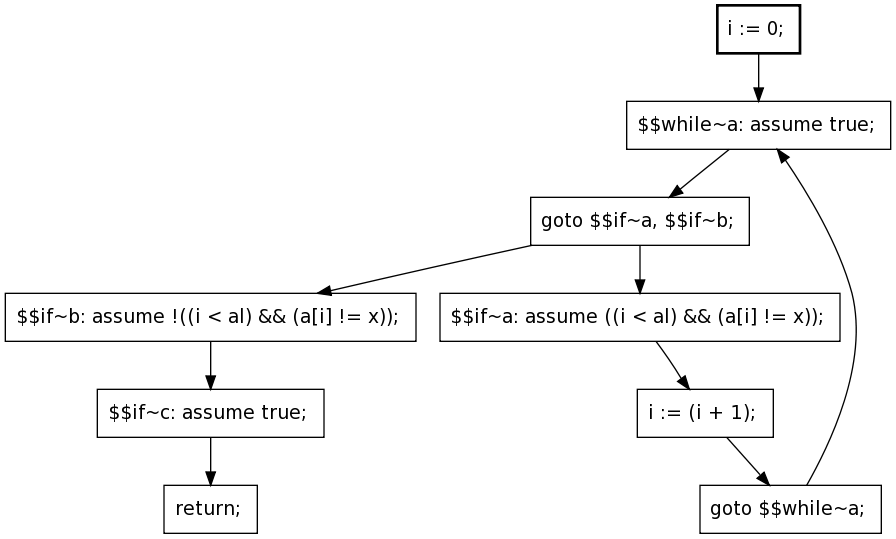
\includegraphics[width=\textwidth]{img/first_boogie.png}
\caption{Flowgraph of a desugared version of Figure~\ref{lst:first-boogie}}
\label{fig:first-boogie}
\end{figure}

The flowgraph is an example of \emph{auxiliary} information that
FreeBoogie computes after each transformation. The other pieces
of auxiliary information are the symbol table and the types. The
\emph{symbol table} is a one-to-many bidirectional map between
identifier definitions and identifier uses. The \emph{types} are
associated with expressions (and subexpressions).

To see the query that is sent to the theorem prover you must
run a different command, this time shown in abbreviated form:
\shell{fb -lf=example.log -ll=info -lc=prover example.bpl} The
log file \texttt{example.log} will contain everything sent to
the prover. The result of the whole run is \shell{OK: indexOf at
example.bpl:2:11} indicating that the program is correct.

%}}}
%{{{sec:pipeline
\section{Pipeline}
\label{sec:pipeline}

Figure~\ref{fig:architecture} shows that FreeBoogie has a
pipeline architecture. The \colorbox{green!50!white}{light green}
color stands for the Boogie AST (\fb abstract \fb syntax \fb
tree); the \colorbox{blue!50!black}{\textcolor{white}{dark blue}}
color stands for the SMT AST\null.

%{{{ fig:architecture
\begin{figure}
  \centering
  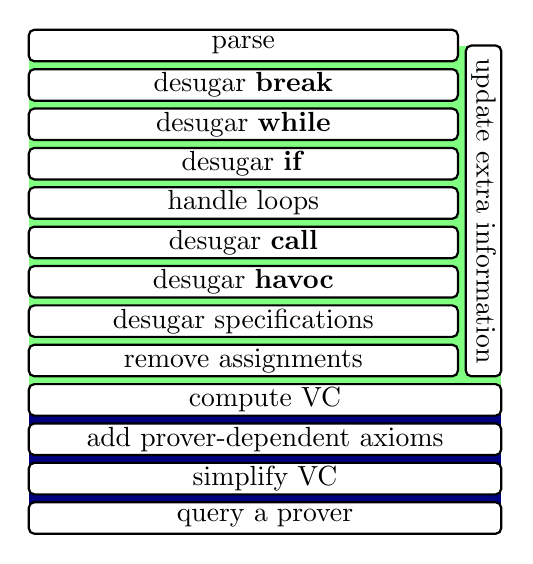
\begin{tikzpicture}[scale=1]
  \tikzstyle phaseS=[thick,rounded corners=2pt,draw=black,fill=white];
  \fill[color=green!50!white] (0,-0.25) rectangle +(6,-4.75);
  \fill[color=blue!50!black] (0,-4.75) rectangle +(6,-1.5);
  \foreach \py/\px/\ptext in {
    0/5.45/parse,
    1/5.45/desugar \textbf{break},
    2/5.45/desugar \textbf{while},
    3/5.45/desugar \textbf{if},
    4/5.45/handle loops,
    5/5.45/desugar \textbf{call},
    6/5.45/desugar \textbf{havoc},
    7/5.45/desugar specifications,
    8/5.45/remove assignments,
    9/6/compute VC,
    10/6/add prover-dependent axioms,
    11/6/simplify VC,
    12/6/query a prover}
  {
    \draw[phaseS]
     [yscale=.5](0,-\py-0.1) rectangle node {\ptext}  +(\px,-.8);
  }
  \draw[phaseS] (5.55,-0.25) rectangle node[rotate=-90] 
    {update extra information} (6,-4.45);

  \end{tikzpicture}
  \caption{FreeBoogie architecture.}
  \label{fig:architecture}
\end{figure}
%}}} fig:architecture

Horizontal boxes, except for the first one (parse) and the last
one (query a prover), represent \emph{transformations}. Depending
on the type of input and on the type of output there are three
types of transformations: Boogie to Boogie, Boogie to SMT, and
SMT to SMT\null. For brevity, we say `Boogie transformations'
instead of `Boogie to Boogie transformations', and `SMT
transformations' instead of `SMT to SMT transformations'. All
these transformations are designed not to miss bugs, at the cost
of possible false positives.

\begin{definition}
A Boogie transformation is \emph{sound} when it produces only
incorrect Boogie programs from incorrect Boogie programs. A
Boogie to SMT transformation is \emph{sound} when it produces
only invalid formulas from incorrect Boogie programs. An SMT
transformation is \emph{sound} when it produces only invalid
formulas from invalid formulas.
\label{def:sound-transform}
\end{definition}

\begin{remark}
This definition is in a way formal, but in a way it is not.
It makes use of the concept of `correct Boogie program'
and we only have semantics for \emph{core} Boogie programs
(Chapter~\ref{ch:boogie}). For example, we can say precisely what
it means for the assignment removal transformation to be sound,
because both the input and the output of that transformation are
core Boogie programs; however, we can only informally describe
the preceding transformations as sound.
\end{remark}

The symmetric notion is that of completeness.

\begin{definition}
A Boogie transformation is \emph{complete} when it produces
only correct Boogie programs from correct Boogie programs. A
Boogie to SMT transformation is \emph{complete} when it produces
only valid formulas from correct Boogie programs. An SMT
transformation is \emph{complete} when it produces only valid
formulas from valid formulas.
\label{def:complete-transform}
\end{definition}

All transformations in FreeBoogie are sound; all transformations
in FreeBoogie, except loop handling,

Full Boogie would not be user friendly without high-level
constructs like \textbf{while} statements and \textbf{break}
statements. Many phases in FreeBoogie perform syntactic
desugarings of these constructs. The desugaring is sometimes
local, in the sense that it can be done without keeping track of
an environment, and sometimes it is not. For example, to desugar
the \textbf{break} statement we must keep track of the enclosing
\textbf{while} and \textbf{if} statements; but the desugaring of
a \textbf{havoc} statement does not depend on any surrounding
code.

The most important transformation in FreeBoogie is the
transition from Boogie to SMT\null. The role of preceding Boogie
transformations is to simplify the program to a form on which the
VC is easily computed; the role of subsequent SMT transformations
is to bring the VC to a form that is easily handled by a prover.

The order of Boogie transformations depends on constraints
such as the following. The Boogie to SMT transformation
(`compute VC' in Figure~\ref{fig:architecture}) only handles
the \textbf{assert}, \textbf{assume}, and \textbf{goto}
statements. The Boogie transformation that removes assignments
only handles acyclic flowgraphs. Hence, the flowgraph must
first be transformed into an acyclic one (`handle loops' in
Figure~\ref{fig:architecture}).

The VC uses concepts such as arrays, which may or may not be
known to the prover. In the latter case, axioms that describe
the concept must be added to the VC\null. Finally, the VC is
simplified so that the communication with the prover is
more efficient.

The source code of FreeBoogie, written in Java~6, contains
four packages, which are in one-to-one correspondence with the
following sections.

\begin{itemize}
\item \texttt{freeboogie.ast}: data structures for representing
  Boogie programs and facilities for processing such data structures
\item \texttt{freeboogie.tc}: code that computes auxiliary information
  from a Boogie AST
\item \texttt{freeboogie.vcgen}: the Boogie transformations and
  the Boogie to SMT transformation
\item \texttt{freeboogie.backend}: 
  SMT transformations, 
  data structures for representing SMT, 
  and code for interfacing with the prover
\end{itemize}

%}}} sec:pipeline
%{{{ sec:design.ast
\section{The Abstract Syntax Tree and its Visitors}
\label{sec:design.ast}

The Boogie AST data structures are described using a compact
notation. A subset, corresponding to core Boogie, appears in
Figure~\ref{fig:boogie-absgrm}. AstGen (a helper tool) reads this
description and a code template to produce Java classes. The
approach has advantages and disadvantages. The generated classes
are very similar to each other because they come from the same
template. This means that it is easy to learn their interface.
It also means that it is easier to change all the classes in a
consistent way by changing the template. The compact description
in Figure~\ref{fig:boogie-absgrm} is easier to read than the
corresponding $12$~Java classes. The overall structure of the AST
is easier to grasp. It is also easier to modify, since it takes
far less time to change one or two lines than one or two Java
classes. However, the programmer needs to learn a new language
(the one used in Figure~\ref{fig:boogie-absgrm}) and IDEs are
usually confused by code generators.

\begin{figure}\centering\footnotesize
\begin{verbatim}
Program = Signature! sig, Body! body;
Signature = String! name, [list] VariableDecl args, [list] VariableDecl results;
Body = [list] VariableDecl vars, Block! block;
VariableDecl = String! name, Type! type;
Block = [list] Statement statements; 
Type = enum(Ptype: BOOL, INT) ptype,
Statement :> AssertAssumeStmt, AssignmentStmt, GotoStmt;
AssertAssumeStmt = enum(StmtType: ASSERT, ASSUME) type, 
  [list] Identifier typeArgs, Expr! expr;
AssignmentStmt = [list] OneAssignment assignments;
GotoStmt = [list] String successors;
Identifier = String! id, 
OneAssignment = Identifier lhs, Expr rhs;
\end{verbatim}
\caption{The abstract grammar of core Boogie}\label{fig:boogie-absgrm}
\end{figure}

Another consequence of this approach, which might be seen as a
disadvantage, is that there is no way to add specific code to
specific classes: We are forced to implement operations over the
AST using the visitor pattern~\cite{gamma1995}.

\subsection{The Abstract Grammar Language}

AstGen reads a description of an abstract grammar and a template.
Therefore it understands two languages---the AstGen abstract
grammar language and the AstGen template language. This section
describes the AstGen abstract grammar language, which was already
used in Figure~\ref{fig:boogie-absgrm}. The syntax of the AstGen
abstract grammar language appears in Figure~\ref{grm:astgen}.
(Note that a formal language is used to describe the concrete
syntax of a language that is used to describe the abstract
grammar of a language whose concrete syntax was studied in
Chapter~\ref{ch:boogie} using the same formal language that
we use here in Figure~\ref{grm:astgen}: There is some opportunity
for confusion.)

\startgrammar
  grammar\is rule\*\\
  rule\is composition \| inheritance \| specification\\
  composition\is class \b= members\? \b;\\
  inheritance\is class {\boldmath$:>$} classes\? \b;\\
  specification\is class \b: text \P\\
  member\is tags type \b!\? name\\
  tag\is \b[ \i{id} \b]\\
  type\is \i{id} \| \b{enum} \b( \i{id} \b: ids\? \b)\\
  members\is member (\b, members)\*\\
  tags\is tag (\b, tags)\*\\
  name, class\is \i{id}\\
\stopgrammar{The syntax of the abstract grammar language}{grm:astgen}

The abstract grammar is described by a list of rules. Each
rule starts with the name of the class to which it pertains. A
composition rule continues with an equal sign (\textbf{=}) and a
list of members. An inheritance rule continues with a supertype
sign ({\boldmath$:>$}) and a list of subclasses. A specification rule
continues with a colon (\textbf{:}) and some arbitrary text. The
end of composition and inheritance rules is marked by a semicolon
(\textbf{;}) and the end of a specification rule is marked by the
end of the line (depicted as \P\ in Figure~\ref{grm:astgen}).
That is (almost) all.

To illustrate why this notation is beneficial, suppose that
initially the data structures for the Boogie AST contained only
public fields.
\begin{jml}
public class Program {
  public Signature sig;
  public Body body;
}
\end{jml}
This Java code is obviously not much longer and indeed very
similar to the first line in Figure~\ref{fig:boogie-absgrm}.
But it has a number or problems. First, we probably want the
\textit{Program} class to be final. Without using AstGen
we must go and add the keyword \textbf{final} in each
class: \textit{Program}, \textit{Signature}, \textit{Body},
\textit{VariableDecl}, $\ldots$ With AstGen, we only need to add
that keyword in the template. Another problem is that there is no
constructor. Again, adding constructors is a repetitive job if we
must do it in each and every class. Finally, FreeBoogie's data
structures are immutable. More precisely, the members are private
and final, they are set by the constructor, and accessor methods
only allow them to be read. Again, making these changes in all
classes is a repetitive job. In summary, the main advantage of
using AstGen is that we separate the concern of defining the
shape of the abstract grammar from lower-level concerns such as
whether we allow subclassing or not, whether we allow mutations
or not.

Specification rules, which refer to classes, and tags, which
refer to members (see Figure~\ref{grm:astgen}), allow for a
little non-uniformity between generated classes. The bang
sign (\textbf{!}) is a shorthand for the tag [nonnull]. As we
will see, the code template may contain parts that are used
or not by AstGen depending on whether a tag is present. In
particular, FreeBoogie's code template asserts nonnullness only
for members with the tag [nonnull]. The only other tag used in
Figure~\ref{fig:boogie-absgrm} is [list], which will be discussed
briefly in Section~\ref{sec:design.immutability}.

A specification rule associates some arbitrary text to a class.
Templates then instruct AstGen where in the output to insert
the arbitrary text. For example, in FreeBoogie the arbitrary
text is always a side-effect free Java boolean expression.
FreeBoogie's code template inserts these boolean expressions in
Java \textbf{assert} statements within constructors. In general,
the intended use of specification rules is to give object or
class invariants. However, there is nothing in AstGen to enforce
this use. Hence, specification rules could be abused to insert,
say, custom comments in the header of generated classes.

\subsection{AstGen Templates}

Figure~\ref{fig:astgen-template} illustrates the main
characteristics of an AstGen template and, at the same time,
gives some details on how the Boogie AST data structures
are implemented. The language for templates is influenced
by \TeX~\cite{knuth1986tex}. Macros start with a backslash
(\macro{}) and may take arguments. Some macros are primitive and
some are defined using \macro{def}. Before cataloging primitive
macros, let us analyze the high-level structure of the template
in Figure~\ref{fig:astgen-template}.

\begin{figure}\centering\footnotesize
\begin{verbatim}
\def{smt}{\if_primitive{\Membertype}{\MemberType}}
\def{mt}{\if_tagged{list}{ImmutableList<}{}\smt\if_tagged{list}{>}{}}
\def{mtn}{\mt \memberName}
\def{mtn_list}{\members[,]{\mtn}}

\classes{\file{\ClassName.java}
/* ... package specification and some imports ... */
public \if_terminal{final}{abstract} class \ClassName extends \BaseName {
\if_terminal{
  \members{private final \mtn;}
  private \ClassName(\mtn_list) {
    \members{this.\memberName = \memberName;}
    checkInvariant();
  }
  public static \ClassName mk(\mtn_list) {
    return new \ClassName(\members[,]{\memberName});
  }
  public void checkInvariant() {
    assert location != null;
    \members{\if_tagged{nonnull|list}{assert \memberName != null;}{}}
    \invariants{assert \inv;}
  }
  \members{public \mtn() { return \memberName; }}
  @Override public <R> R eval(Evaluator<R> evaluator) { 
    return evaluator.eval(this); 
  }
}{
  \selfmembers{public abstract \mtn();}
}} }
\end{verbatim}
\caption{Excerpt from the AstGen template for Boogie AST classes}
\label{fig:astgen-template}
\end{figure}

The first four lines define macros that are used later. AstGen
then sees the (primitive) \macro{classes} macro and processes its
argument once for each class in the abstract grammar. Terminal
classes, those that have no subclass declared in the abstract
grammar, have private fields, a private constructor that
initializes those fields, a static factory method \textit{mk}, a
method \textit{checkInvariant}, accessors for getting the values
of the fields, and a method \textit{eval}, which is typically
called \textit{accept} in most presentations of the visitor
pattern. Non-terminal classes only have abstract accessors for
getting the values of the fields.

The primitive macros can be grouped in four categories:
(1)~output selection, (2)~data, (3)~test, and (4)~iteration.

The macro \macro{file}\{\thinspace\textit{f}\} globally directs
the output from now on to the file~\textit{f}.

The data macros do not take any parameter. They expand to the
name of the current class (\macro{className}), the name of the
base class of the current class (\macro{baseName}), the type
of the current member (\macro{memberType}), the name of the
current member (\macro{memberName}), the name of the current
enumeration (\macro{enumName}), the current enumeration value
(\macro{valueName}), the current invariant (\macro{inv}).
The `current' class\slash member\slash enumeration\slash
value\slash invariant is determined by the enclosing iteration
macros. All data macros except \macro{inv} are made of two
words and they come in four case conventions (camelCase,
PascalCase, lower\_case, and UPPER\_CASE): The output is
formatted accordingly.

The test macros have the shape
\macro{if}\textit{condition}\{\textit{yes}\}\{\textit{no}\}.
If the condition holds then the \textit{yes} part is processed
and the \textit{no} part is ignored; if the condition does not
hold then the \textit{no} part is processed and the \textit{yes}
part is ignored. The braces in the \textit{yes} and \textit{no}
parts must be balanced. The condition \texttt{\_primitive}
holds when the type of the current member does not appear on
the left hand side of a composition rule. (In particular,
it holds for members whose type is an enumeration.) The
condition \texttt{\_enum} holds when the type of the current
member is an enumeration. The condition \texttt{\_terminal}
holds when the current class has no subclass. The condition
\texttt{\_tagged$\{$\textrm{\textit{tag\_expression}}$\}$}
is more interesting. A tag expression may contain tag names,
logical-and (\texttt{\&}), logical-or (\texttt{|}), and
parentheses. A tag name evaluates to \textbf{true} when the current
member has that tag.

The iteration macros have the shape
\macro{}\textit{macro}[\textit{separator}]\{\textit{argument}\}.
The argument is processed repeatedly and the optional separator
is copied to the output between two passes over the argument. The
macro \macro{classes} processes its argument for each class (and
hence each pass has a `current class'). The macro \macro{members}
processes its argument for each member of the current class,
including inherited members (and hence each pass has a `current
member'). The macro \macro{selfmembers} processes its argument
for each member of the current class, excluding inherited
members (and hence each pass has a `current member'). The macro
\macro{invariants} processes its argument for each invariant of
the current class, which appear in specification rules (and hence
each pass has a `current invariant'). The macro \macro{enums}
processes its argument for each enumeration used as a type in the
current class (and hence each pass has a `current enumeration').
The macro \macro{values} processes its argument for each value
of the current enumeration (and hence each pass has a `current
enumeration value').

It is an error for a macro~$x$ to appear in a context where
there should be a current~$y$, but there is none. For example,
it is an error for the macro \macro{enumName} to appear in a
context where there is no current enumeration. In other words,
the macro \macro{enumName} cannot appear outside of the argument
of \macro{enums}, which is the only macro that sets a current
enumeration.


\subsection{Visitors}
\label{sec:visitors}

The visitor pattern is widely used to implement compilers. It can
be seen as a workaround to a limitation of most object-oriented
languages. A reference~$u$ has the static type~$C_u$ when the
declaration of variable~$u$ is \jmlCode|$C_u$ u;| a reference~$u$
has the dynamic type~$C'_u$ when it points to an object whose
type is~$C'_u$; an object has the type~$C'_u$ when it was created
by the statement \jmlCode|new $C'_u$($\cdots$)|. The method call
\jmlCode|u.m(v)| is resolved based on the dynamic type~$C'_u$
and on the static type~$C_v$. In other words, the code that will
be executed is in a method named~$m$ that takes an argument
of type~$C_v$ (or a supertype of~$C_v$) and is defined in the
class~$C'_u$ (or a supertype of~$C'_u$). There is no way to
do the dispatch based on the dynamic type of two (or more)
references.

However, it is possible to do the dispatch based on the
dynamic types of~$n$ references \emph{one by one}, at the
cost of writing extra code. Say the references $u_1$,~$u_2$,
\dots,~$u_n$ have static types $C_1$,~$C_2$, \dots,~$C_n$ and
dynamic types $C'_1$,~$C'_2$, \dots,~$C'_n$. The initial call
\jmlCode|$u_1$.$u_1$($u_2$,$\ldots$,$u_n$)| will execute a method
\jmlCode|$m_1$($C_2,\ldots,C_n$)| from the class~$C'_1$, because
all the (proper) subclasses of $C_1$ implement such a method. The
body of all these methods will be identical: It will contain the
call \jmlCode|$u_2$.$m_2$(this, $u_3,\ldots,u_n$)|. Each subclass
of~$C_2$, including $C'_2$, is expected to have a \emph{set}
of methods \jmlCode|$m_2$($\mathscr{C}_1,C_3,C_4,\ldots,C_n$)|
for all possible (proper) subclasses~$\mathscr{C}_1$
of~$C_1$. The static type of \jmlCode|this| in the call
\jmlCode|$u_2$.$m_2$(this, $u_3,\ldots,u_n$)| was~$C'_1$, so the
method with $\mathscr{C}_1=C'_1$ will be chosen out of the whole
set. In general, all subclasses of~$C_k$ must implement a set of
methods \jmlCode|$m_k$.($\mathscr{C}_1,\ldots,\mathscr{C}_{k-1},
C_{k+1},\ldots,C_n$)|, for all subclasses~$\mathscr{C}_1$
of~$C_1$, all subclasses~$\mathscr{C}_2$ of~$C_2$, and so on. The
methods~$m_n$ will do the actual work. Let us estimate the number
of methods that only forward calls and were referred to in the
beginning of the paragraph as `extra code'. If the number of
possible types for $u_1$,~$u_2$, \dots,~$u_n$ is, respectively,
$w_1$,~$w_2$, \dots,~$w_n$ then the number of methods $m_k$ is
$\prod_{i\le k} w_i$. There are therefore $\sum_{k<n}\prod_{i\le
k} w_i$ methods whose only purpose is forwarding and $\prod_{i\le
n} w_i$ methods that do something interesting.

As is traditionally presented, the visitor pattern is the case
$n=2$ with $C_1$ being the root of the AST class hierarchy and
$C_2$ being the root of the visitors class hierarchy. There is
exactly one forwarding method per AST class (and their total
number is $w_1$ with the previous notation). In this guise,
the visitor pattern can be seen as a way of grouping together
the code that achieves one conceptual operation. For example,
pretty printing an AST can be done by implementing a method
\textit{prettyPrint} in each AST class, but can also be done by
putting all the pretty printing code into one visitor called
\textit{PrettyPrinter}. (Note that AstGen makes it hard to use
the former approach, with a specific \textit{prettyPrint} method
in each class.)

FreeBoogie uses the traditional visitor pattern and
the root of the visitors' class hierarchy is the class
\jmlCode|Evaluator<R>|. The root of the Boogie AST
class hierarchy is the class \jmlCode|Ast|. A subclass
of \jmlCode|Evaluator<R>| is like a function of type
$\mathit{Ast}\to R$, in the sense that it associates a
value of type~$R$ (possibly \jmlCode|null|) to an AST
node. For example, the type checker is a subclass of
\jmlCode|Evaluator<Type>|. The base class \jmlCode|Evaluator|
declares one \jmlCode|eval($\mathscr{A}$)| method for each AST
class~$\mathscr{A}$. These are the methods called~$m_2$ in the
previous discussion of the general visitor pattern. These methods
are not only declared, but they are also implemented, so that
subclasses explicitly handle only the relevant types of AST
nodes. For all the other AST node types, the default behavior
implemented in \jmlCode|Evaluator| is to recursively evaluate all
children and to cache the results. Because the \jmlCode|eval|
methods of \jmlCode|Evaluator| are so similar, they are generated
from an AstGen template.

An important type of evaluator is a transformer: The class
\jmlCode|Transformer| extends \jmlCode|Evaluator<Ast>|. The
main functionality implemented in \jmlCode|Transformer|, path
copying, is illustrated in Figure~\ref{fig:path-copying}. Empty
nodes (\tikz[baseline=-.5ex] \node[fgdraw,circle] {}; and
\tikz[baseline=-.5ex] \node[fgdraw]{};) represent AST nodes
that exist on the heap before a transformer~$T$ acts; filled
nodes (\tikz[baseline=-.5ex] \node[fgdraw,fgfill,circle]{};
and \tikz[baseline=-.5ex] \node[fgdraw,fgfill]{};) represent
AST nodes created by the transformer~$T$. Because the
transformer~$T$ is interested only in rectangle nodes,
it overrides only the \jmlCode|eval| method that takes
rectangles as parameters. That overriden method is responsible
for creating the filled rectangle (\tikz[baseline=-.5ex]
\node[fgdraw,fgfill]{};). All the other filled nodes
(\tikz[baseline=-.5ex] \node[fgdraw,fgfill,circle]{};) are
created by \textit{Transformer}, and need not be of any concern
to the particular transformer~$T$.

\begin{figure}\centering
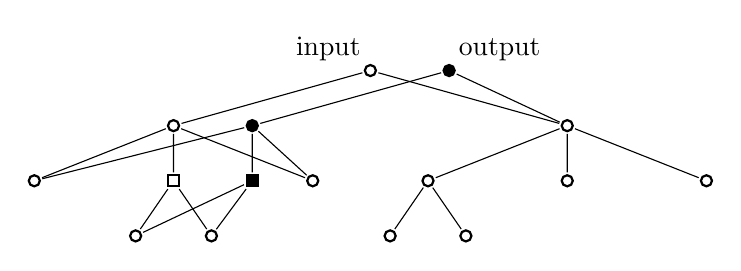
\begin{tikzpicture}
  [level distance=7mm,
  level/.style={sibling distance=5cm/(#1^1.5)}]
\tikzset{tree/.style={fgdraw,circle}}
\node[tree] (A) {}
  child {node[tree] (B) {}
    child {node[tree] (B1) {}}
    child {node[tree,rectangle] (C) {}
      child {node[tree] (C1) {}}
      child {node[tree] (C2) {}}
    }
    child {node[tree] (B3) {}}
  }
  child {node[tree] (A2) {}
    child {node[tree] {}
      child {node[tree] {}}
      child {node[tree] {}}
    }
    child {node[tree] {}}
    child {node[tree] {}}
  };
\path
  (A) +(1cm,0) node[tree,fgfill] (A') {}
  (B) +(1cm,0) node[tree,fgfill] (B') {}
  (C) +(1cm,0) node[tree,fgfill,rectangle] (C') {};
\draw (A') -- (B') -- (C');
\draw (A') -- (A2);
\draw (B') -- (B1); \draw (B') -- (B3);
\draw (C') -- (C1); \draw (C') -- (C2);
\node[above left] at (A) {input};
\node[above right] at (A') {output};
\end{tikzpicture}
\caption{Path copying}\label{fig:path-copying}
\end{figure}

The input and the output of a transformer usually share a large
number of nodes. Since \textit{Evaluator} caches the information
that various evaluators associate with AST nodes, there is no
need to repeat the computation of that auxiliary information for
the shared parts. For example, most of the type information is
already in the cache of the type checker.

Sometimes a transformer wants to `see' AST nodes of type~$A$
even if it computes no value for them. A typical example is
a pretty printer. In such cases a transformer may override
\jmlCode|eval(A)| and return \textbf{null}. A nicer solution is
to override \jmlCode|see(A)|, whose return type is \textbf{void}.
If both \jmlCode|eval(A)| and \jmlCode|see(A)| are overriden,
then the former will be called by the traversal code in
\textit{Transformer}.


\subsection{Immutability}
\label{sec:design.immutability}

In Java programming, it is unusual to constrain data structures
to be immutable. Since the resulting code may look awkward to
many programmers, there better be some good reasons for this
design decision. In fact, awkward code, such as copying all but
one of the fields in a new object instead of doing a simple
assignment, is only one of the apparent problems.

\bc
\begin{jml}
public class Renamer extends Transformer {
  @Override public Identifier eval(Identifier identifier) {
    if (!identifier.id().equals("u")) return identifier;
    else return Identifier.mk("v");
  }
}
\end{jml}
\ec{Changing all occurrences of variable~$v$ into variable~$y$}
{lst:example-transformer}

Immutability implies path copying, which is a
potential performance problem. Consider the task of
changing all occurrences of the variable~$u$ into
variable~$v$, which is achieved by the transformer in
Figure~\ref{lst:example-transformer}. Suppose an AST with
height~$h$ and $n$~nodes contains exactly one occurrence of
variable~$u$. If the class \textit{Identifier} would be mutable,
one assignment would be enough to achieve the substitution;
since the class \textit{Identifier} is immutable, about $h$ new
nodes must be created and initialized. However, if there are
two occurrences of variable~$u$, they share some ancestors,
meaning that less than about $2h$ new AST nodes must be created
and initialized. Even more, if we take into account the tree
traversal, then both implementations, with a mutable AST and with
an immutable AST, take $\Theta(n)$ time. In other words, there is
no asymptotic slowdown.

A Boogie block contains a \emph{list} of statements (see
Figure~\ref{fig:boogie-absgrm}). Such lists should be immutable,
but there are no immutable lists in the Java API (\fb application
\fb programming \fb interface), only immutable \emph{views} of
lists. Immutable collections can be implemented such that
immutability is enforced statically by the compiler or such
that immutability is enforced by runtime checks. Unfortunately,
the former is incompatible with implementing Java API
interfaces~\cite{javaCollectFaq}. For example, in order to use
the iteration statement
\jmlCode|for (T x : xs)|,
one must implement the interface \textit{Iterable} that
contains the method \textit{remove}. Obviously, calls to
the \textit{remove} method are not prevented statically by
the compiler. FreeBoogie uses the \textit{ImmutableList}
class from the Google Collections~\cite{google-collect}
library, which follows the approach with runtime checks.
(Figure~\ref{fig:astgen-template} shows that the
\textit{ImmutableList} is used whenever the [list] tag appears in
the abstract grammar.)

However, the advantages of immutability outweigh its
disadvantages.

First, immutability enables \textit{Evaluator} to cache the
results of previous computations, because only immutable data
structures can be used as keys in maps. A particular evaluator,
such as the type-checker, need not mention anywhere in its
implementation that caching is used. Yet, if the type-checker
is invoked twice on the same AST fragment, then the second call
will return immediately. This leads to cleaner code also because
AST transformers need not bother with updating the auxiliary
information---recomputing it is cheap. These advantages are
discussed further in Chapter~\ref{ch:ev}.

Second, immutability makes the code easier to understand, because
it frees the programmer from thinking about aliasing of AST nodes.
In Java, any mutation of \jmlCode|u.f| must be done only after
thinking how it will affect code that uses possible aliases of~$u$.
Because the AST is a central data structure in FreeBoogie, there
is a lot of potential aliasing that must be considered whenever
a mutation is done. It is much simpler to forbid mutations altogether.

Still, there are situations when the programmer must think about
aliasing of AST data structures. It is natural to think of an
AST reference as \emph{being} a piece of a Boogie program,
even if, strictly speaking, it only \emph{represents} a piece
of a Boogie program. To maintain this useful illusion the
programmer must ensure that no sharing occurs within one version
of the AST\null. More precisely, there should never be more
than one reference-paths between two AST nodes. (There is a
\emph{reference-edge}~$u\to v$ from the object referred by~$u$
to the object referred by~$v$ when \jmlCode|u.f==v| for some
field~$f$.) For example, if the expression~$x+y$ appears multiple
times in a Boogie program, then the corresponding AST also
appears multiple times, instead of being shared. In practice,
this means that the programmer must occasionally clone pieces
of the AST when implementing transformers. (The \textit{clone}
method is implemented in the code template for AST classes.)

%}}} sec:design.ast
%{{{ aux
\section{Auxiliary Information}

The package \textit{freeboogie.tc} derives extra information from
a Boogie AST---types, a symbol table, and a flowgraph.

The AST constructed by the parser is type-checked in order to
catch simple mistakes in the input. As a safeguard against bugs,
the AST is type-checked after each transformation. A side-effect
of type-checking is that the type of each expression is known.

The symbol table helps in navigating the AST\null. It consists of
one-to-many bidirectional maps that link identifier declarations
to places where the identifiers are used. The only such
map that is relevant to core Boogie is the one that links
variable declarations, including those in arguments, to uses
of variables. The other maps, relevant to full Boogie, link
procedure declarations to procedure calls, type declarations to
uses of user defined types, function declarations to uses of
(uninterpreted) functions, and type variables to uses of type
variables. (Type variables are similar to generics in Java.) All
these maps are in the class \textit{SymbolTable}.

Another bidirectional map is built by
\textit{ImplementationChecker}: In full Boogie a \emph{procedure}
may have zero, one, or multiple \emph{implementations}. (In core
Boogie, the whole program is one implementation.)

Finally, it is sometimes convenient to view one implementation as
a flowgraph whose nodes are statements. Such a flowgraph is built
by \textit{FlowGraphMaker}. Formally, a flowgraph is defined as
follows.

\begin{definition}
A \emph{flowgraph} is a directed graph with a distinguished
\emph{initial node} from which all nodes are reachable.
\end{definition}

It seems natural that a flowgraph has an initial node, because
there is usually one entry point to a program. It seems less
natural that all nodes must be reachable, which means that
there is no obviously dead code. The reason for this standard
restriction is rather technical: It simplifies the study of
flowgraph properties. However, it does complicate slightly the
definition of what it means for a flowgraph to correspond to a
core Boogie program. A few terminology conventions will help. In
Chapter~\ref{ch:boogie} we noticed that we can attach counters
to statements because they are in a list. For concreteness, let
us use the counters $1$,~$2$ \dots, $n$, in this order, when the
list of statements has length~$n$. Each counter~$x$ in the range
$0.\,.\>n$ has an associated statement, named statement~$x$.
Statement~$0$ is the sentinel statement \textbf{assume true},
which is prepended for convenience. Label~$x$ is the label that
precedes statement~$x$, if there is one.

\begin{remark}
The sentinel statement~$0$ is not introduced by the FreeBoogie
implementation. It is merely a device that will simplify the
subsequent presentation, especially some proofs.
\end{remark}

The flowgraph of a Boogie program is constructed, conceptually,
in two phases.

\begin{definition}
The \emph{pseudo-flowgraph of a core Boogie program} with
$n$~statements has as nodes statement~$1$ up to statement~$n$
and the sentinel statement~$0$. It has an edge~$0\to1$
(from statement~$0$ to statement~$1$) and has edges~$x\to
y$ when (a)~statement~$x$ is \textbf{goto} label~$y$, or
(b)~statement~$x$ is \emph{not} \textbf{goto} and label~$y$ is
the successor of label~$x$.
\end{definition}

\begin{remark}
Compare with
\eqref{eq:assume-assert-ok-opsem}--\eqref{eq:goto-opsem}.
This definition roughly says that there is an edge where the
operational semantics rules would allow a transition \emph{if we
ignore the upper parts of the rules}.
\end{remark}

\begin{definition}
The \emph{flowgraph of a core Boogie program} is a graph that has
node~$0$ as its initial node. Its nodes~$V$ are those nodes of
the pseudo-flowgraph that are reachable from node~$0$ and that
are not \textbf{goto}~statements. It has an edge~$m\to n$ when
there is a path~$m\leadsto n$ in the pseudo-flowgraph that is
disjoint from~$V$, except at endpoints.
\label{def:boogie-flowgraph}
\end{definition}

\begin{example}
Figure~\ref{fig:boogie-flowgraph} shows a core Boogie program,
its pseudo-flowgraph, and its flowgraph. (Label~$k$ is $L_k$.)
Chapter~\ref{ch:reachability} discusses \emph{semantically}
unreachable nodes of the flowgraph, such as node~$4$ in this
example.
\end{example}

\begin{proposition}
The only nodes that have no outgoing edges in a flowgraph of a
core Boogie program are those that correspond to \textbf{return}
statements.
\end{proposition}

\begin{figure}
\centering
\begin{tabular}{ccc}
\begin{boogie}[boxpos=c]
procedure dead(x : int) returns () {
  $L_1$: assume x > 0;
  $L_2$: goto $L_4$, $L_6$;
  $L_3$: assume true;
  $L_4$: assume x < 0;
  $L_5$: return;
  $L_6$: assume true;
  $L_7$: return;
}
\end{boogie}&
\hspace{5mm}
\begin{tikzpicture}[scale=.5,baseline=0.75cm]
  \foreach \n/\x/\y in {0/1/4, 1/1/3, 3/3/4, 4/0/1, 5/0/0, 6/2/1, 7/2/0}
    \oonode (\n) at (\x,\y) [label=left:$\n$] {};
  \node[fgdraw] (2) at (1,2)  [label=left:$2$] {};

  \foreach \i/\j in {0/1, 1/2, 2/4, 2/6, 4/5, 6/7}
    \draw[arr] (\i) -- (\j);
\end{tikzpicture}&
\hspace{5mm}
\begin{tikzpicture}[scale=.5,baseline=0.5cm]
  \foreach \n/\x/\y in {0/1/3, 1/1/2, 4/0/1, 5/0/0, 6/2/1, 7/2/0}
    \oonode (\n) at (\x,\y) [label=left:$\n$] {};
  \foreach \i/\j in {0/1, 1/4, 1/6, 4/5, 6/7}
    \draw[arr] (\i) -- (\j);
\end{tikzpicture}
\\
\end{tabular}
\caption{Flowgraph of a core Boogie program}\label{fig:boogie-flowgraph}
\end{figure}

All auxiliary information is available through
\textit{TcInterface}, which is an implementation of the Facade
pattern.

%}}} aux
%{{{ vcgen
\section{Verification Condition Generation}

The package \textit{freeboogie.vcgen} consists of Boogie
transformers and Boogie to SMT transformers. The facade of this
package is the class \textit{VcGenerator}.

Most Boogie transformers are responsible for small AST
modifications such as desugaring an \textbf{if} statement
into \textbf{assume} and \textbf{goto} statements. For speed,
it would be better to cluster many such simple transformers
into one, but the code is easier to maintain if they are kept
separate. A few helper classes are used by multiple Boogie
transformers: \textit{CommandDesugarer} is used as a base class
by transformers that change statements into lists of statements;
\textit{ReadWriteSetFinder} is an evaluator that associates with
each statement two sets---the set of variables that are read and
the set of variables that are written.

Boogie transformations do not update the auxiliary information
while they are building new AST nodes. Instead, at the very end,
they recompute all auxiliary information, and caches ensure that
no computation is repeated. This way, bugs that produce untypable
Boogie programs get caught at run-time. (Type information is
auxiliary information, so type-checking is repeated.)

The Boogie to SMT transformation is done by the
class \textit{WeakestPrecondition} or by the class
\textit{StrongestPostcondition}, depending on the command line
options. The theory behind these two classes is presented in
Chapter~\ref{ch:spwp}.

%}}} vcgen
% {{{ sec:design.backend
\section{The Prover Backend}
\label{sec:design.backend}

The package \textit{freeboogie.backend} contains (1)~SMT data
structures and (2)~code to communicate with provers. The design
is inspired by the sorted multi-prover backend in \escjava.

\subsection{Data Structures and Sort-Checking}
\label{sec:design.ds}

The main data structure is a rooted ordered tree whose nodes are
labeled by strings. Each node has a \emph{sort}, and there are
sort-checking rules, which say what combinations of sorts and
labels are valid. In effect, sorts are types---the only reason a
different name is used is to distinguish SMT sorts from
Boogie types. In \escjava it is impossible to construct a tree
that has sort errors: Programs that try to construct invalid
terms fail Java type-checking. Such a strong static guarantee is
appealing, but has a significant disadvantage: The size of the
backend is big. For example, instead of a single factory method
  \jmlCode|SmtTree mk(String label, ImmutableList<SmtTree> children)|
there is a plethora of methods with various argument and return
types, such as the method
  \jmlCode|SmtFormula mkEq(SmtTerm left, SmtTerm right)|,
where both \textit{SmtFormula} and \textit{SmtTerm} are subtypes
of \textit{SmtTree}. Because of the size, the backend is hard to
adapt to changes. FreeBoogie opts for dynamic checks instead of
static guarantees so that the backend is smaller and easier to
maintain.

Before calling \jmlCode|mk(label, children)| the label must have
been defined. For example, after the call
  \jmlCode|def("eq", new Sort[]{Sort.TERM, Sort.TERM}, Sort.FORMULA)|
it is possible to call
  \jmlCode|mk("eq", children)|.
This second call will check (using Java assertions) that there are
two children and both are terms, and will mark the constructed
SMT tree as being a formula. All defined labels are grouped in
stack frames, such that the call \jmlCode|popDef()| discards
all definitions done after the corresponding call \jmlCode|pushDef()|.
Such grouping is useful because some labels refer to constructs
built into SMT solvers and other labels refer to uninterpreted
functions that are defined by the Boogie program. When
FreeBoogie moves from one input file to another it forgets about
labels corresponding to functions while not forgetting about
labels corresponding to solver built-ins by using the stack
mechanism.

The methods \textit{def}, \textit{mk}, \textit{pushDef}, and
\textit{popDef} are all defined in the class \textit{TreeBuilder}.
For convenience, the functions \textit{def} and \textit{mk} are
overloaded.

Let us first look at the method~\textit{mk}. It comes in three
varieties:
\begin{align}
&\text{\jmlCode|mk("and", children)|}\\
&\text{\jmlCode|mk("eq", $t_1$, $t_2$)|}\\
&\text{\jmlCode|mk("literal_int", new FbInteger(3))|}
\end{align}
The first form takes a list of children as the second
argument. When the number of children is fixed, as is the
case for the label \texttt{eq}, it is convenient to hide the
building of the list behind a helper overload. The second form
can be used when the number of children is one, two, or three.
The third form is special. Strictly speaking, the constants
$1$,~$2$, $3$~$\ldots$ are distinct uninterpreted functions
that take no argument. This suggests that they should each
be defined separately, which is clearly a very bad idea from
the point of view of performance. So, instead of defining
labels \texttt{1},~\texttt{2}, \texttt{3},~\dots, we define
the meta-label \texttt{literal\_int}. A \emph{meta-label} has
an associated Java type (in this case \textit{FbInteger}) and
it is equivalent to multiple labels, one for each value of the
associated Java type. In other words, the meta-label 
\texttt{literal\_int} and the value \jmlCode|new FbInteger(3)|
determine the label, and there is no child.

Now let us look at the method~\textit{def}. It comes in three
varieties:
\begin{align}
&\text{\jmlCode|def("and", Sort.FORMULA, Sort.FORMULA)|}\\
&\text{\jmlCode|def("eq", new Sort[]\{Sort.TERM, Sort.TERM\}, Sort.FORMULA)|}\\
&\text{\jmlCode|def("literal_int", FbInteger.class, Sort.INT)|}
\end{align}
The order of the arguments is: label, sort of arguments, sort
of result. The example for the first form says that tree nodes
labeled with \texttt{and} may have any number of children, all of whom
must be formulas, and the tree itself is a formula. The example
for the second form says that tree nodes labeled \texttt{eq} have
two children, the first one is a term, the second one is a term,
and the tree itself is a formula. The example for the third form
says that the meta-label \texttt{literal\_int} together with a
value of type \textit{FbInteger} constitutes a label, and trees
labeled in this way are integers.

(As a side note, \textit{FbInteger} is used because Boogie allows
arbitrary large integers and has bit vector operations. No class
in the standard Java library supports both.)

Any SMT trees $s$ and~$t$ have the property that
\jmlCode|s.equals(t)| implies \jmlCode|s==t|. This is implemented
by maintaining a global set of all SMT trees that were created, a
technique sometimes known by the name \emph{hash-consing}.

\subsection{The Translation of Boogie Expressions}

The methods \textit{mk} provide one way of building trees; the
method~\textit{of} provides another way of building trees.
For example, the class \textit{StrongestPostcondition} uses
the methods~\textit{mk} to connect formulas (using the labels
\texttt{and}, \texttt{implies}) and uses the method~\textit{of}
to obtain the formulas corresponding to individual assertions and
assumptions.

The method~\textit{of} converts from Boogie expressions
to SMT formulas. The actual work is done in two
classes---\textit{TermOfExpr} and \textit{FormulaOfExpr}. The
translation is almost one-to-one. Each Boogie operator has a
corresponding interpreted symbol in the SMT language; each
function declared in a (full) Boogie program behaves similarly
to an uninterpreted function symbol in the SMT language.
There is, however, an important deviation from the one-to-one
correspondence. As we have seen, the SMT language distinguishes
between terms and formulas. Roughly speaking these correspond,
respectively, to non-boolean Boogie expression and to boolean
Boogie expressions. For example, in the SMT language the
operands of logical-and must be formulas and in Boogie the
operands of logical-and must be booleans. On the other hand, an
SMT uninterpreted symbol is always a term, while in Boogie a
function may return a boolean. Also, in SMT the arguments of an
uninterpreted symbol must be terms, while in Boogie a function
might take booleans as arguments. Because of these reasons, a
one-to-one translation may produce ill-formed SMT trees, which
fail sort-checking.

In SMT the constants \textbf{true} and \textbf{false} are a
formulas. If we introduce two corresponding uninterpreted terms,
\textit{trueTerm} and \textit{falseTerm}, we can then try to fix
the ill-formed SMT tree using the following two rules.
\begin{enumerate}
\item If a term~$\tau$ appears where a formula is expected then we 
  replace the term by \smtCode|(= $\tau$ trueTerm)|. This compares
  for equality $\tau$ and \textit{trueTerm}.
\item If a formula~$\varphi$ appears where a term is expected
  then we replace the formula by 
  \smtCode|(ite $\varphi$ trueTerm falseTerm)|.
  This expression evaluates to \textit{trueTerm} for all 
  interpretations in which $\varphi$~evaluates to \textbf{true};
  it evaluates to \textit{falseTerm} for all interpretations
  in which $\varphi$~evaluates to \textbf{false}.
\end{enumerate}
This, however, is not exactly what FreeBoogie does.
Simplify is an old but still competitive prover whose language is
similar to the SMT language. One difference is that in Simplify
a term never contains a formula. In particular, there is no
\textbf{ite}, so the rule~2 from above cannot be used.

To clarify these ideas, let us turn to an example.
\begin{boogie}
function f(x : bool) returns (bool);
axiom (forall x : bool :: x == f(x));
procedure p() returns () { assert f(true) != f(false); }
\end{boogie}
The assertion should hold. 

The following is what FreeBoogie sends to Simplify.
\begin{smt}
(BG_PUSH (NEQ trueTerm falseTerm))
(BG_PUSH (FORALL (xTerm) (EQ xTerm (f xTerm))))
(NOT (IFF (EQ trueTerm (f trueTerm) (EQ trueTerm (f falseTerm)))))
\end{smt}

In Simplify's language, interpreted symbols are written
in \textsc{capital} letters and their names are usually
self-explanatory. The command \textbf{BG\_PUSH} communicates a
hypothesis to the prover. Line~3 is a query. The Boogie constants
\textbf{true} and \textbf{false} that appear as arguments
of the function~$f$ were translated into terms directly,
without an intermediate application of rule~2. The comparison
between booleans~\boogieCode|$\bullet$ != $\bullet$|, which appears
in the assertion, was translated to \smtCode|(NOT (IFF $\bullet$ $\bullet$))|. 
Because \textbf{IFF} expects formulas as arguments and because
\smtCode|(f $\ldots$)| is a term, rule~1 was applied, which is
why \textbf{EQ} appears in the query.

The hypothesis on line~1 is necessary. In fact, it is equivalent
to the query.
\begin{align*}
&\qquad\text{\smtCode|(NOT (IFF (EQ trueTerm (f trueTerm) (EQ trueTerm (f falseTerm)))))|}\\
&\text{= \{\thinspace instantiate hypothesis 2 with $\mathit{xTerm}=\mathit{trueTerm}$\thinspace\}}\\
&\qquad\text{\smtCode|(NOT (IFF TRUE (EQ trueTerm (f falseTerm)))))|}\\
&\text{= \{\thinspace boolean algebra\thinspace\}}\\
&\qquad\text{\smtCode|(NEQ trueTerm (f falseTerm))|}\\
&\text{= \{\thinspace \smtCode|(f falseTerm)| is the same as \textit{falseTerm}, again from hypothesis 2\thinspace\}}\\
&\qquad\text{\smtCode|(NEQ trueTerm falseTerm)|}
\end{align*}

The example illustrates that it is sometimes necessary to
introduce new hypotheses. If not enough hypotheses are
introduced, then FreeBoogie is incomplete, but should still be
sound. Whenever \textit{TermOfExpr} or \textit{FormulaOfExpr}
produce an SMT tree, they may attach to it extra hypotheses.
These are SMT trees themselves, and may have further hypotheses
attached. All hypotheses are collected and sent to the prover
before the query.


\subsection{Talking to the Prover}

The class \textit{Prover} defines the interface that is used
by the package \textit{freeboogie.vcgen} to talk to the
prover. It is a thin interface, consisting of the methods
\textit{assume}, \textit{retract}, \textit{push}, \textit{pop},
and \textit{isValid}.

The real prover does not have to have the notion of an
assumption (also known as hypothesis), but a class that extends
\textit{Prover} should take advantage of all facilities of a real
prover. For example, if Simplify is used as a prover, then a
sequence of calls \jmlCode|assume(h)|, \jmlCode|isValid($q_1$)|,
\jmlCode|isValid($q_2$)| may result in one of the following two
strings being sent to the prover:
\begin{align}
&(\mathbf{IMPLIES}\;h\;q_1)\;(\mathbf{IMPLIES}\;h\;q_2)\\
&(\mathbf{BG\_PUSH}\;h)\;q_1\;q_2
\end{align}
Both are OK, but the second is better, if only because
$h$ is communicated once.

Similarly, a class that extends \textit{Prover} may choose to
treat certain SMT tree labels specially to take advantage of
other facilities of the real prover.

%}}} sec:design.backend
%{{{ gencode
\section{Other Generated Code}

The Boogie parser resides in the package
\textit{freeboogie.parser} and is generated by ANTLR
(\textbf{an}other \fb tool for \fb language \fb
recognition); the command line parser resides in the package
\textit{freeboogie.cli} and is generated by CLOPS (\fb command
\fb line \textbf{op}tion\textbf{s}).

%}}} gencode
%{{{ related
\section{Related Work}

The main goal of the previous sections is to anchor the
subsequent theoretical chapters in a concrete program,
FreeBoogie. A secondary goal is to serve as a guide to the code
and to make explicit the early design choices. This section is
for the reader who wants to understand the design in detail, but
feels that the previous sections are too shallow.

\subsection{Similar Tools}

FreeBoogie is a Java clone of the Boogie
tool~\cite{barnett2005boogie} from Microsoft Research. The
internals differ but the input and the output interfaces
are the same. The input is a program written in the Boogie
language~\cite{leino2008boogie,leino2010boogie}; the output is a
formula written in the SMT language, or in a similar language.

The Boogie language is imperative. The Why
language~\cite{filliatre2007why} is functional and, like
Boogie, was designed to be an intermediate language for program
verifiers. The Why language is used by the Why tool.

Since both the Boogie tool and the Why tool accomplish tasks
similar to FreeBoogie, it is interesting to compare their design
decisions. For example, it is easy to see that they were written
in different programming languages. Both Boogie and FreeBoogie
can be used to verify themselves. The Boogie tool is written in
\specsharp, a superset of \csharp, and is part of a verification
system~\cite{barnett2005spec} for \specsharp programs. FreeBoogie
is written in Java and can be used to verify Java programs if it
is combined with the converter B2BPL from Java bytecode to Boogie
that was developed at ETH Z\"urich. (The source code of B2BPL
is included in the FreeBoogie code repository.) In the case of
the Why tool, however, the choice of language was not governed
by such recursive considerations: It is written in OCaml, a
language well suited for implementing compilers, but it is not
used to verify OCaml code. The main use of the Why tool is in
the Jessie plugin of the Frama-C framework~\cite{framac} for
the verification of C programs. Similarly, it is interesting to
compare approaches to representing ASTs, interfacing with provers
(Why being especially interesting), and so on.

\subsection{Design, Pipeline, and Correctness}

Because the input and the output are programs written in
well-defined languages, FreeBoogie is a compiler. The standard
text on compiler design is the Dragon Book~\cite{aho2007}. The
pipeline architecture is common to most compilers.

One of the oldest problems studied by the formal methods
community is the correctness of compilers. The early approaches
were focused on proving that a compiler is correct (see, for
example, \cite{moore1989cc}). The idea is to show that the
semantics of the input program are in a certain relationship
with the semantics of the output program. The relationship
usually ensures that the two programs have the same observable
behavior. Although there is recent research in the same
vein~\cite{leroy2009}, there are also attempts to go around the
problem and avoid the full verification of the compiler. One of
these alternative approaches is \emph{translation validation},
proposed in 1998 by Amir Pnueli and others~\cite{pnueli1998tv}.
The idea is to check the result of each particular compilation,
instead of proving that the compiler works for all possible
inputs. To make it even easier, instead of checking the whole
compilation, the idea can be applied to each compilation phase.
The technique was used to find bugs in GCC (the \fb GNU \fb
C \fb compiler)~\cite{necula2000tv}. A related technique,
\emph{credible compilation}~\cite{rinard1999credible}, consists
of modifying the compiler to output a proof for each compilation.
It if then possible to check the proof of equivalence using a
small trusted proof checker. In 2004, Benton~\cite{benton2004}
introduced a way of doing equivalence proofs that seems to
fit well with the Boogie language.

The problem of correctness of a program verifier has certain
peculiarities. The `observable behavior' of a Boogie program,
which is not executable, is whether it is correct or not,
according to Definition~\ref{def:correctness}. It follows that
two Boogie programs are equivalent if they are both correct or
both incorrect. As with normal compilers, a transformation of
a Boogie program is correct if the output is equivalent to the
input. Section~\ref{sec:pipeline} says that some transformations
in FreeBoogie are incorrect and it identifies soundness and
completeness as weaker guarantees.

The Dragon Book analyzes the problem of correctness from an
algorithmic point of view, but it does not address the problem
of correctness of an implementation; the Dragon Book discusses
the overall pipeline architecture of a compiler but does not
go into details of code organization. The Design Patterns
book~\cite{gamma1995} partly covers this area. For example, the
visitor pattern, the facade pattern, and the factory method
pattern, which were used to explain FreeBoogie's design, are all
presented in that book. Of these three patterns, only the visitor
pattern was briefly analyzed in Section~\ref{sec:visitors}.

``[A] \emph{facade} provide[s] a unified interface to a set
of interfaces in a subsystem. Facade defines a higher-level
interface that makes the subsystem easier to use.'' In this
dissertation a more specific meaning is used---a class (or
interface) that provides almost all the services of a package.
The non-facade classes are still visible from outside, in case
they are needed, but their use is discouraged.

A \emph{factory method} creates an object and returns it. The
Design Patterns book emphasizes that the method call may be
dynamically dispatched to subclasses. While this aspect is used
by the backend, the factory methods for Boogie AST are static.
Such methods lead to code that is easier to read because of their
descriptive names and because Java's type inference for generics
works better for methods than for constructors, at least in
version~6. Such methods also make possible the implementation
of more sophisticated creation patterns, such as singleton and
hash-consing.

\subsection{The Expression Problem}

The visitor pattern is a way of achieving multiple dynamic
dispatch, but it is also a partial solution to the
expression problem. The term was coined by Philip Wadler in an
email~\cite{wadler1998ep} from 1998: ``The \emph{Expression
Problem} is a new name for an old problem. The goal is to define
a datatype by cases, where one can add new cases to the datatype
and new functions over the datatype, without recompiling existing
code, and while retaining type safety.'' Since most languages
have modular compilation, the restriction on recompilation
usually means that one is allowed to add new modules but not to
modify existing ones. Wadler continues: ``One can think of cases
as rows and functions as columns in a table. In a functional
language the rows are fixed [$\ldots$] but it is easy to add new
columns. In an object-oriented language, the columns are fixed
[$\ldots$] but it is easy to add new rows.''

The visitor pattern is a way of easily adding new columns in
an object-oriented language. In compilers, functionality tends
to evolve more than the AST. This is one reason why functional
languages are well-suited for implementing compilers and it is
why most compilers written in object oriented languages use the
visitor pattern. However, once the visitor pattern is used, it
becomes hard to modify the AST.

FreeBoogie is written in an object oriented language and uses
the visitor pattern. To add new functionality, one implements a
new evaluator or a new transformer, both being visitors. The
code implementing the new functionality goes in a new class so,
in Wadler's terminology, it is easy to add columns. If a new
type of node must be added to the AST then one new class must
be added to the AST data structures. So far, the existing code
was not touched and no recompilation is necessary. The next
step, however, is to add a methods to \textit{Evaluator}, the
root of the hierarchy of visitors. In Wadler's terminology, it
is hard to add rows. What is problematic in practice is not the
recompilation time, but the fact that the AST data structures
and the base classes for visitors must be kept in sync. Because
the AST data structures, the class \textit{Evaluator}, and the
class \textit{Transformer} are generated by AstGen from the same
description of the abstract grammar they are \emph{automatically}
in sync. In other words, AstGen can be seen as a patch that
brings the visitor pattern closer to the ideal solution for the
expression problem. (But recompilation is still necessary when
new AST nodes are added.)

Another approach to the expression problem is to
modify the programming language to support multiple
dispatch~\cite{chambers1994mm,clifton2006}.

\subsection{Provers}

Many languages understood by theorem provers (such as the SMT
language, the Simplify language, and the PVS prover language)
are based on S-expressions. Like XML~\cite{bray2006xml} (the
e\textbf{x}tensible \fb markup \fb language), S-expressions
provide a syntax that is easy to parse. Briefly, they are a fully
parenthesized preorder print of an AST\null. Where XML says
\texttt{<tag>$\,\cdots$</tag>}, S-expressions say \texttt{(tag
\dots)}. (There is no equivalent for XML attributes.) One year
before writing about the semantics of programs, John McCarthy
presented~\cite{mccarthy1960} in 1960 how S-expressions are used
in the programming system LISP (\textbf{lis}t \fb processing).
``S stands for symbolic.''

Internally, FreeBoogie uses a tree of strings to represent
symbolic expressions. To save memory and to speed up otherwise
expensive structural comparisons FreeBoogie uses hash-consing.
The idea was described by Andrei Ershov~\cite{ershov1958} in
1957, and one year later an English translation was available.
Before creating a tree node, a global hash table is searched to
see if a structurally similar node already exists. The creation
of nodes takes a constant amount of time on average, structural
comparison of tree nodes is done then by a simple pointer
comparison, and much memory is saved because duplication of
information is avoided. A simple implementation of hash-consing
is easy, but offering proper library support is not trivial---a
solution~\cite{filliatre2006hash} for OCaml was published
in~2006.

The tree of strings was chosen as the main data
structure of \textit{freeboogie.backend} because it
is a natural representation of the SMT language. The
SMT community~\cite{ranise2009smtlib} produced a
language~\cite{ranise2006smtlang}, a command language,
theories, benchmarks; it also organizes an annual
competition~\cite{barrett2005} between SMT provers. The language
defines, on top of S-expressions, the meaning of about twenty
keywords and about a dozen `attributes'. There are more than a
dozen actively developed provers and more than a dozen other
provers that support the SMT language. The SMT language itself
describes the syntax and semantics of formulas and of terms,
but it does not provide any other way of communicating with the
prover. The SMT command language specifies how to interact with
a running prover---how to ask ``is formula $\varphi$ valid,''
how to say ``from now on please assume $\varphi'$ holds,''
what format the prover should use to answer, and so on. The
theories are the `standard library' of the SMT language. Each
defines the meaning of a set of symbols. For example, the
theory Ints, defines the semantics of the symbols \texttt{0},
\texttt{1}, \texttt{\char`\~}, \texttt{-}, \texttt{+},
\texttt{*}, \texttt{<=}, \texttt{<}, \texttt{>=}, and \texttt{>}.
The benchmarks include hand-crafted queries, random queries,
queries produced from hardware verification tasks, and queries
produced from software verification tasks. A random sample of the
benchmarks is used in the SMT competition. Since the SMT language
is supported by many provers that compete each year on software
verification tasks, it makes a natural target for FreeBoogie.

According to the results of the most recent SMT competition
the best provers are Barcelogic~\cite{bofill2008barcelogic},
Boolector~\cite{brummayer2009boolector},
MathSAT~\cite{bruttomesso2008mathsat}, SatEEn~\cite{sateen},
Yices~\cite{yices}, and Z3~\cite{moura2008z3}. Each of these won
at least one category in~2009. (Although Z3 did not officially
participate, its version from 2008 was still tested and it
unofficially won a few categories.) FreeBoogie was used so
far with \fx~\cite{fx7}, Simplify~\cite{detlefs2005}, and Z3,
which support the slightly different language of Simplify.
Unfortunately, the source code of all the best provers is
not open. \fx and Simplify are open source but not actively
maintained, and are written in esoteric languages whose compilers
are hard to get (Nemerle and Modula~3, respectively).

A better way to interact with provers is through an API\null.
Boolector, MathSAT, Yices, and Z3 provide a C API\null. Z3
provides also a .NET API and an OCaml API\null. Unfortunately,
they are different, since SMT does not define an uniform
API\null.

\subsection{Code Generators}

The Boogie AST is generated by AstGen; the Boogie parser is
generated by ANTLR; the command-line parser is generated by
CLOPS.

ANTLR~\cite{parr1995} is probably the most widely used parser
generator for Java. The grammar is $\mathrm{LL}(k)$, but
backtracking can be optionally activated. FreeBoogie sticks to
$\mathrm{LL}(k)$ so that the generated parser is as fast as
possible. ANTLR can construct AST trees. This facility is not
used. It is not easy to convince ANTLR to generate different
data structures for the AST\null. For example, it is not easy to
convince ANTLR to generate immutable ASTs. Also, it is not easy
to convince ANTLR to generate the root of the visitors' hierarchy
in sync with the AST data structures.

CLOPS~\cite{janota2009clops} is a Java parser generator
specialized for command lines. FreeBoogie is one of its first
users.

There are, of course, other parser generators for Java. ANTLR
was chosen because it is widely used and because a C++ version
of AstGen combined with Bison~\cite{bison} already showed that
the approach is viable. CLOPS was chosen because its authors were
nearby and easy to convince to add new features and fix bugs, if
needed.

%}}} related
\bibliographystyle{plain}
\bibliography{fb}
\end{document}
% vim:spell errorformat=%f\:%l-%m,%f\:%l\:%m,%f\:%m
% vim:textwidth=75
